\documentclass[a4paper]{book}


\usepackage[latin1]{inputenc}    
\usepackage[T1]{fontenc}
\usepackage[francais]{babel}     
\usepackage{hyperref}
\usepackage{graphicx}



\title{Edukera}
\date{12 sept. 2017}
\begin{document}
\maketitle

\section{Acc�der � Edukera}
Tout d'abord, rendez-vous sur \href{https://www.edukera.com/}{le site d'Edukera} (\url{https://www.edukera.com/}).
Au moment o� j"'�crit ces lignes, le site ressemble � cela:

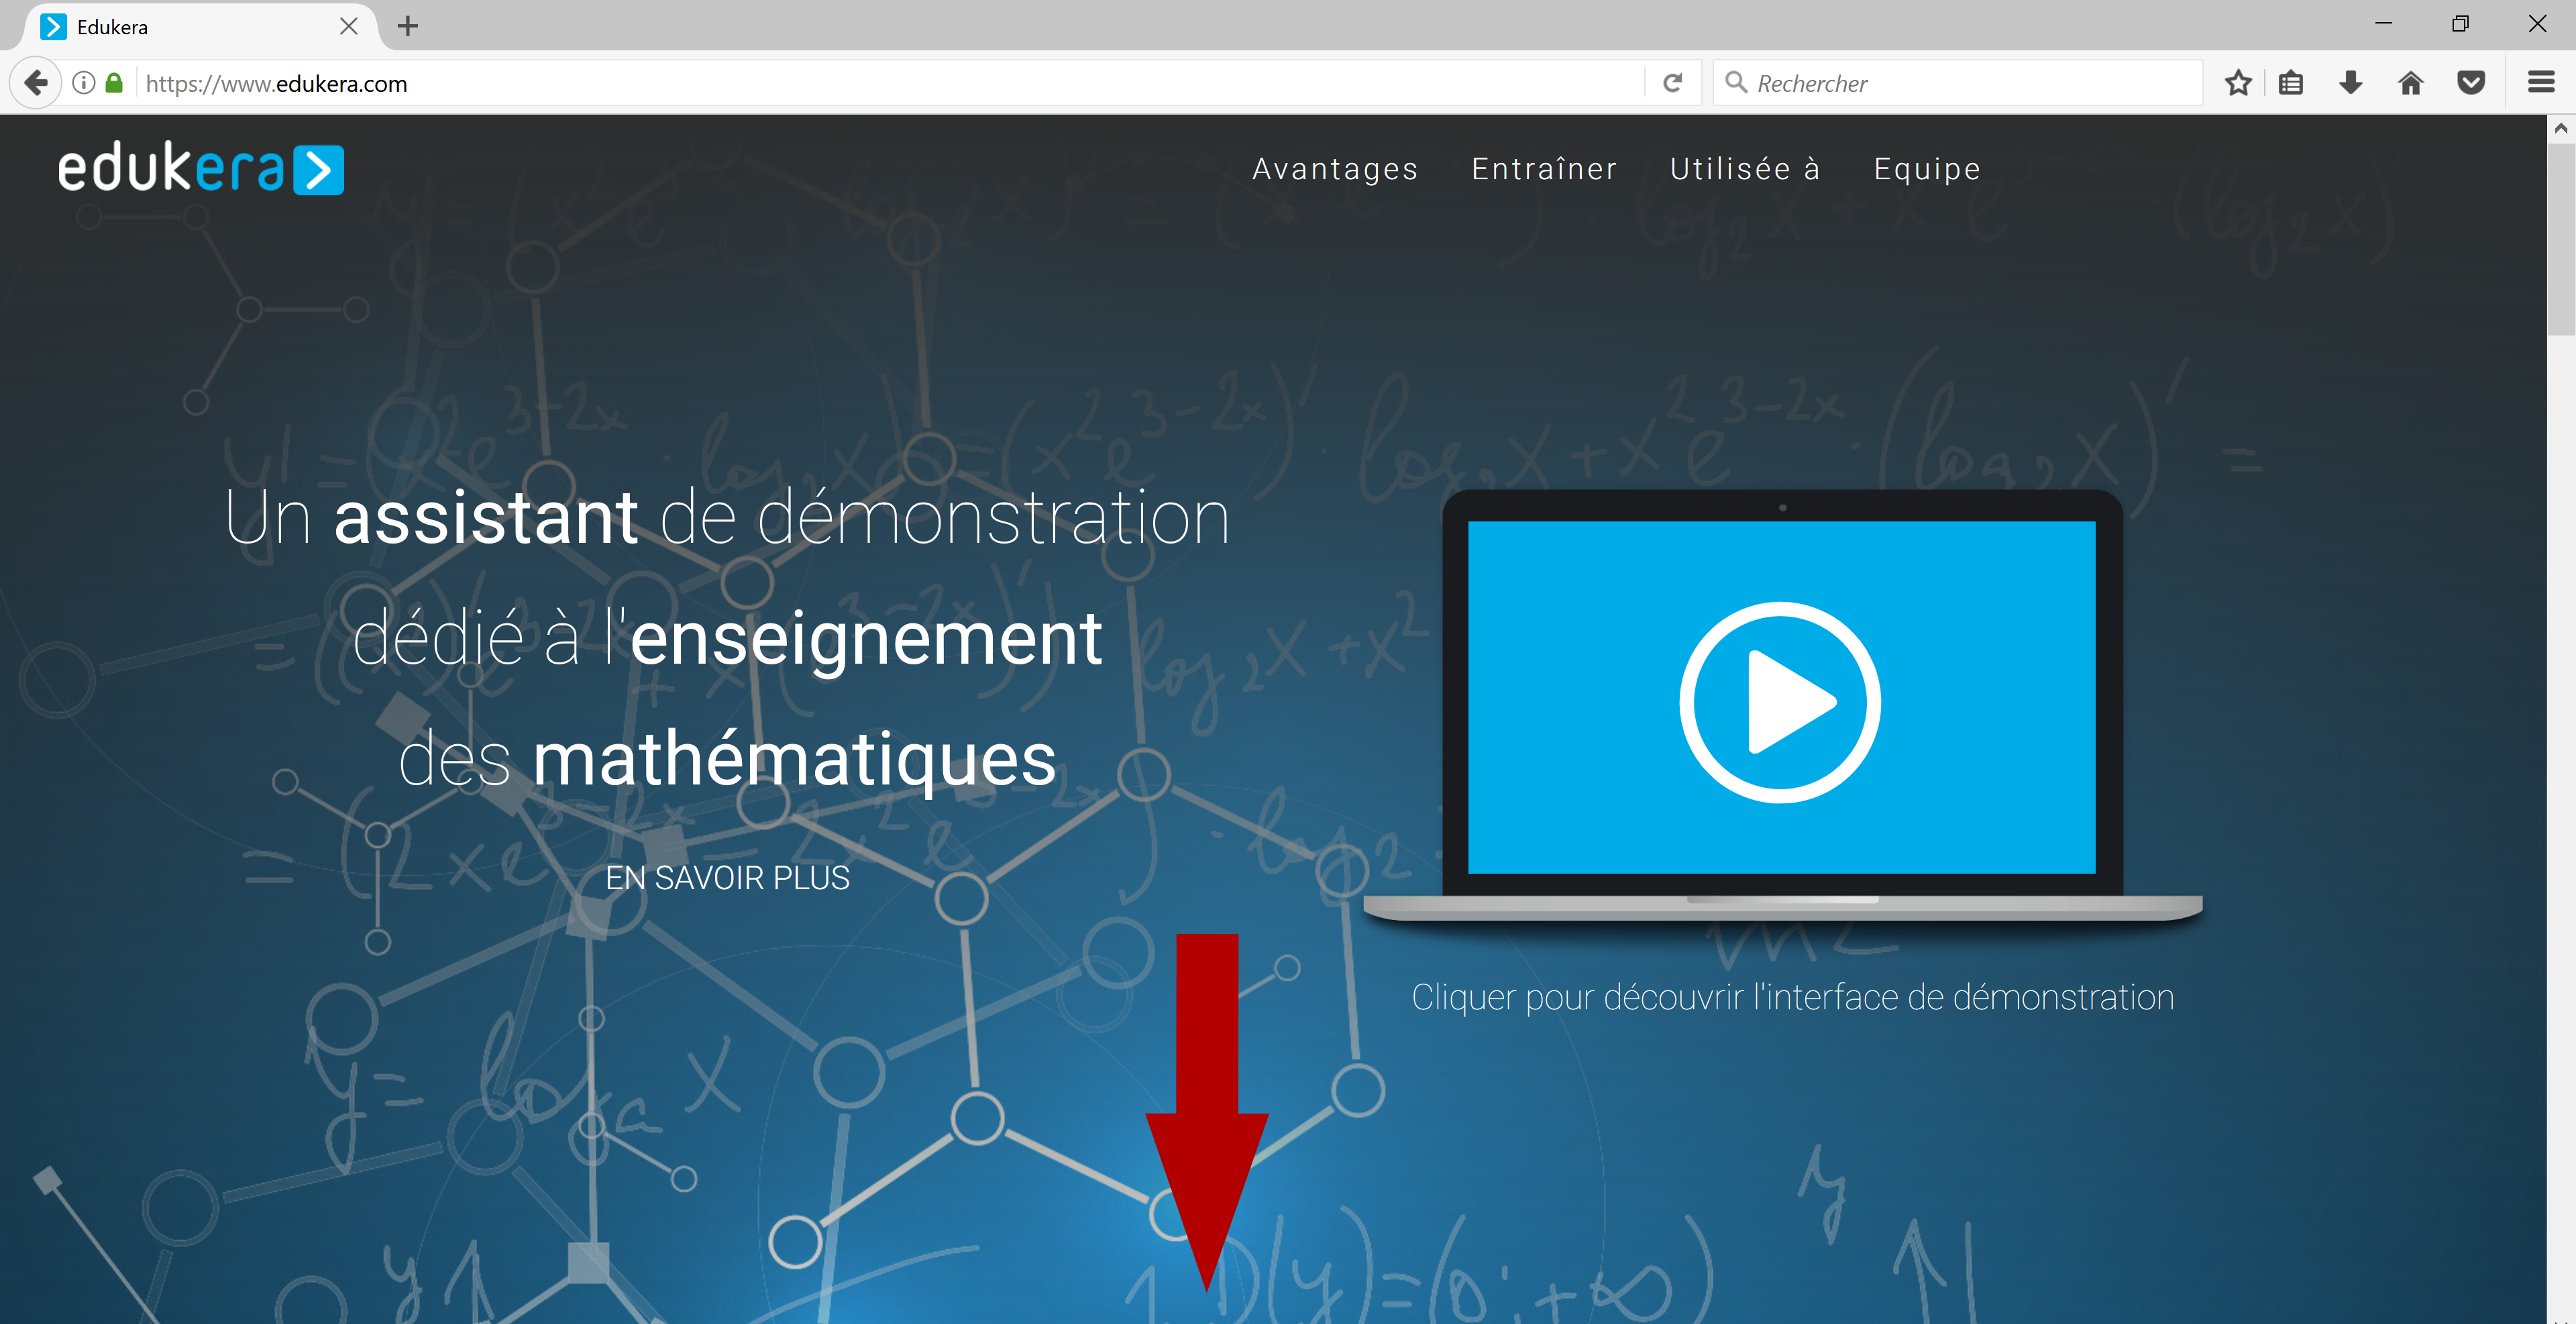
\includegraphics[scale=0.1]{img_site0.png}

Le site fait la promotion d'Edukera, mais ce qui nous int�resse est d'acc�der � l'application. Si vous cliquez sur "d�couvrir l'interface de d�monstration", vous n�acc�derez pas � l'application Edukera, mais � un tutoriel. Pour acc�der � Edukera, faites d�filer le site vers le bas, jusqu'� ce que le bouton "Acc�der � l�application" apparaisse dans le bandeau sup�rieur, comme dans l'image suivante:

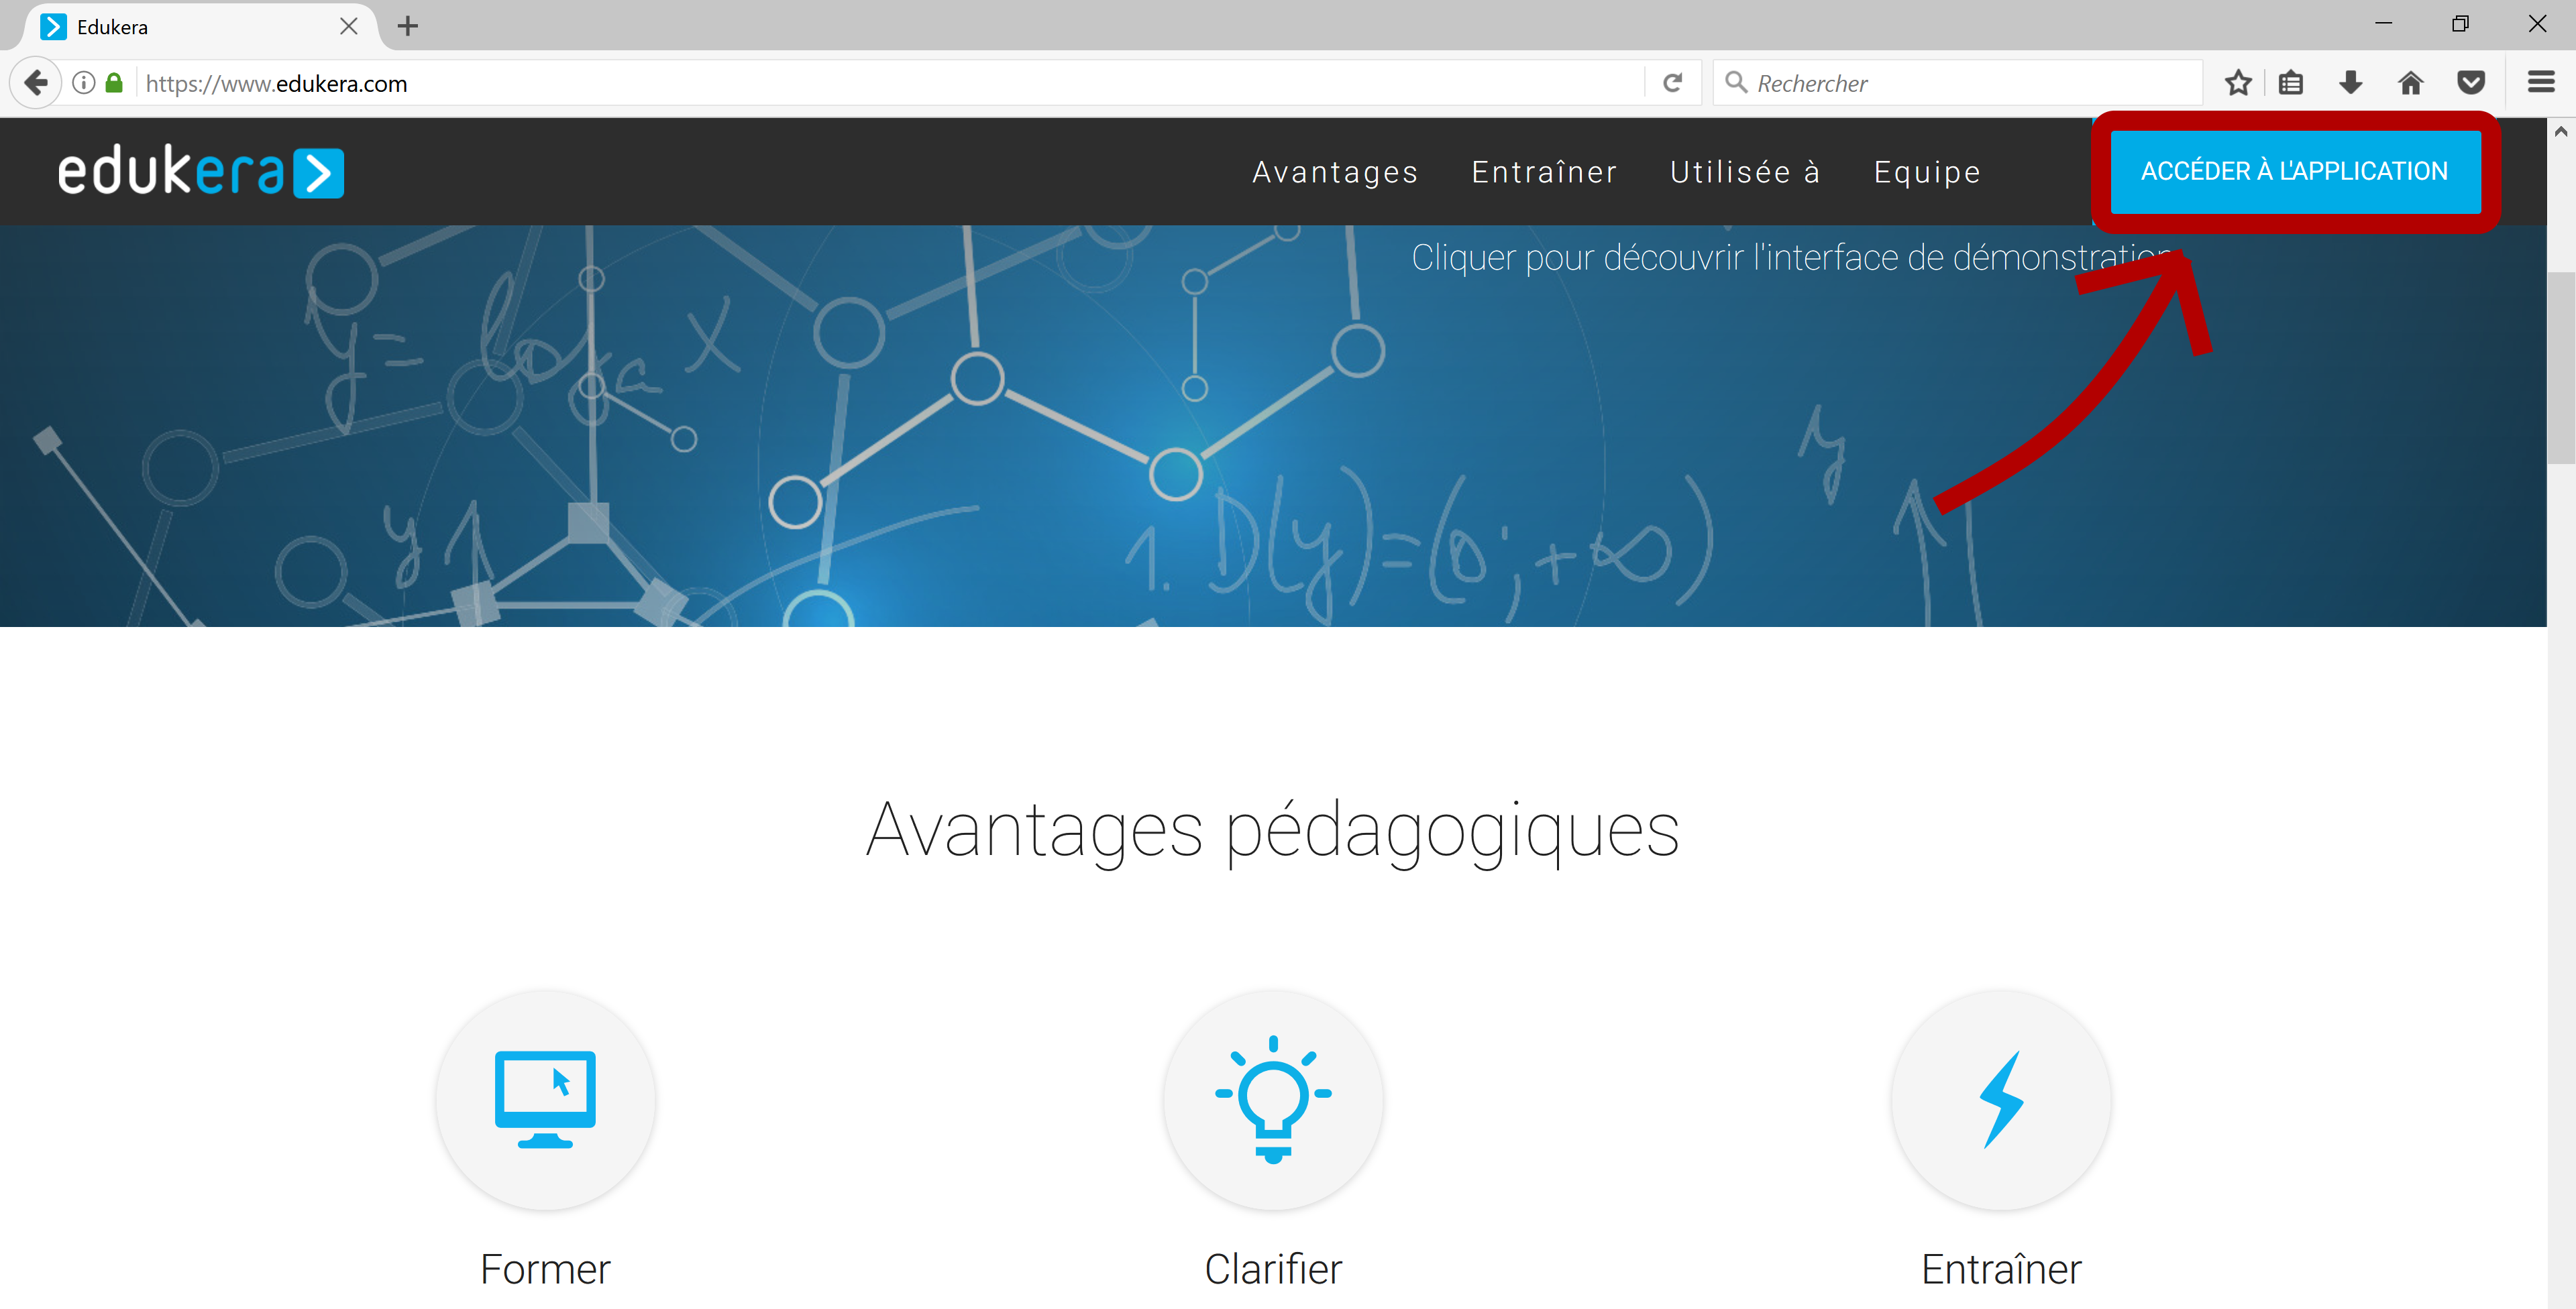
\includegraphics[scale=0.1]{img_site1.png}

Un nouvel onglet va s'ouvrir (l'adresse devrait �tre \url{https://app.edukera.com/}). Vous serez amen�s � cr�er un compte, faites-le. La page de cr�ation de compte devrait ressembler � cela:

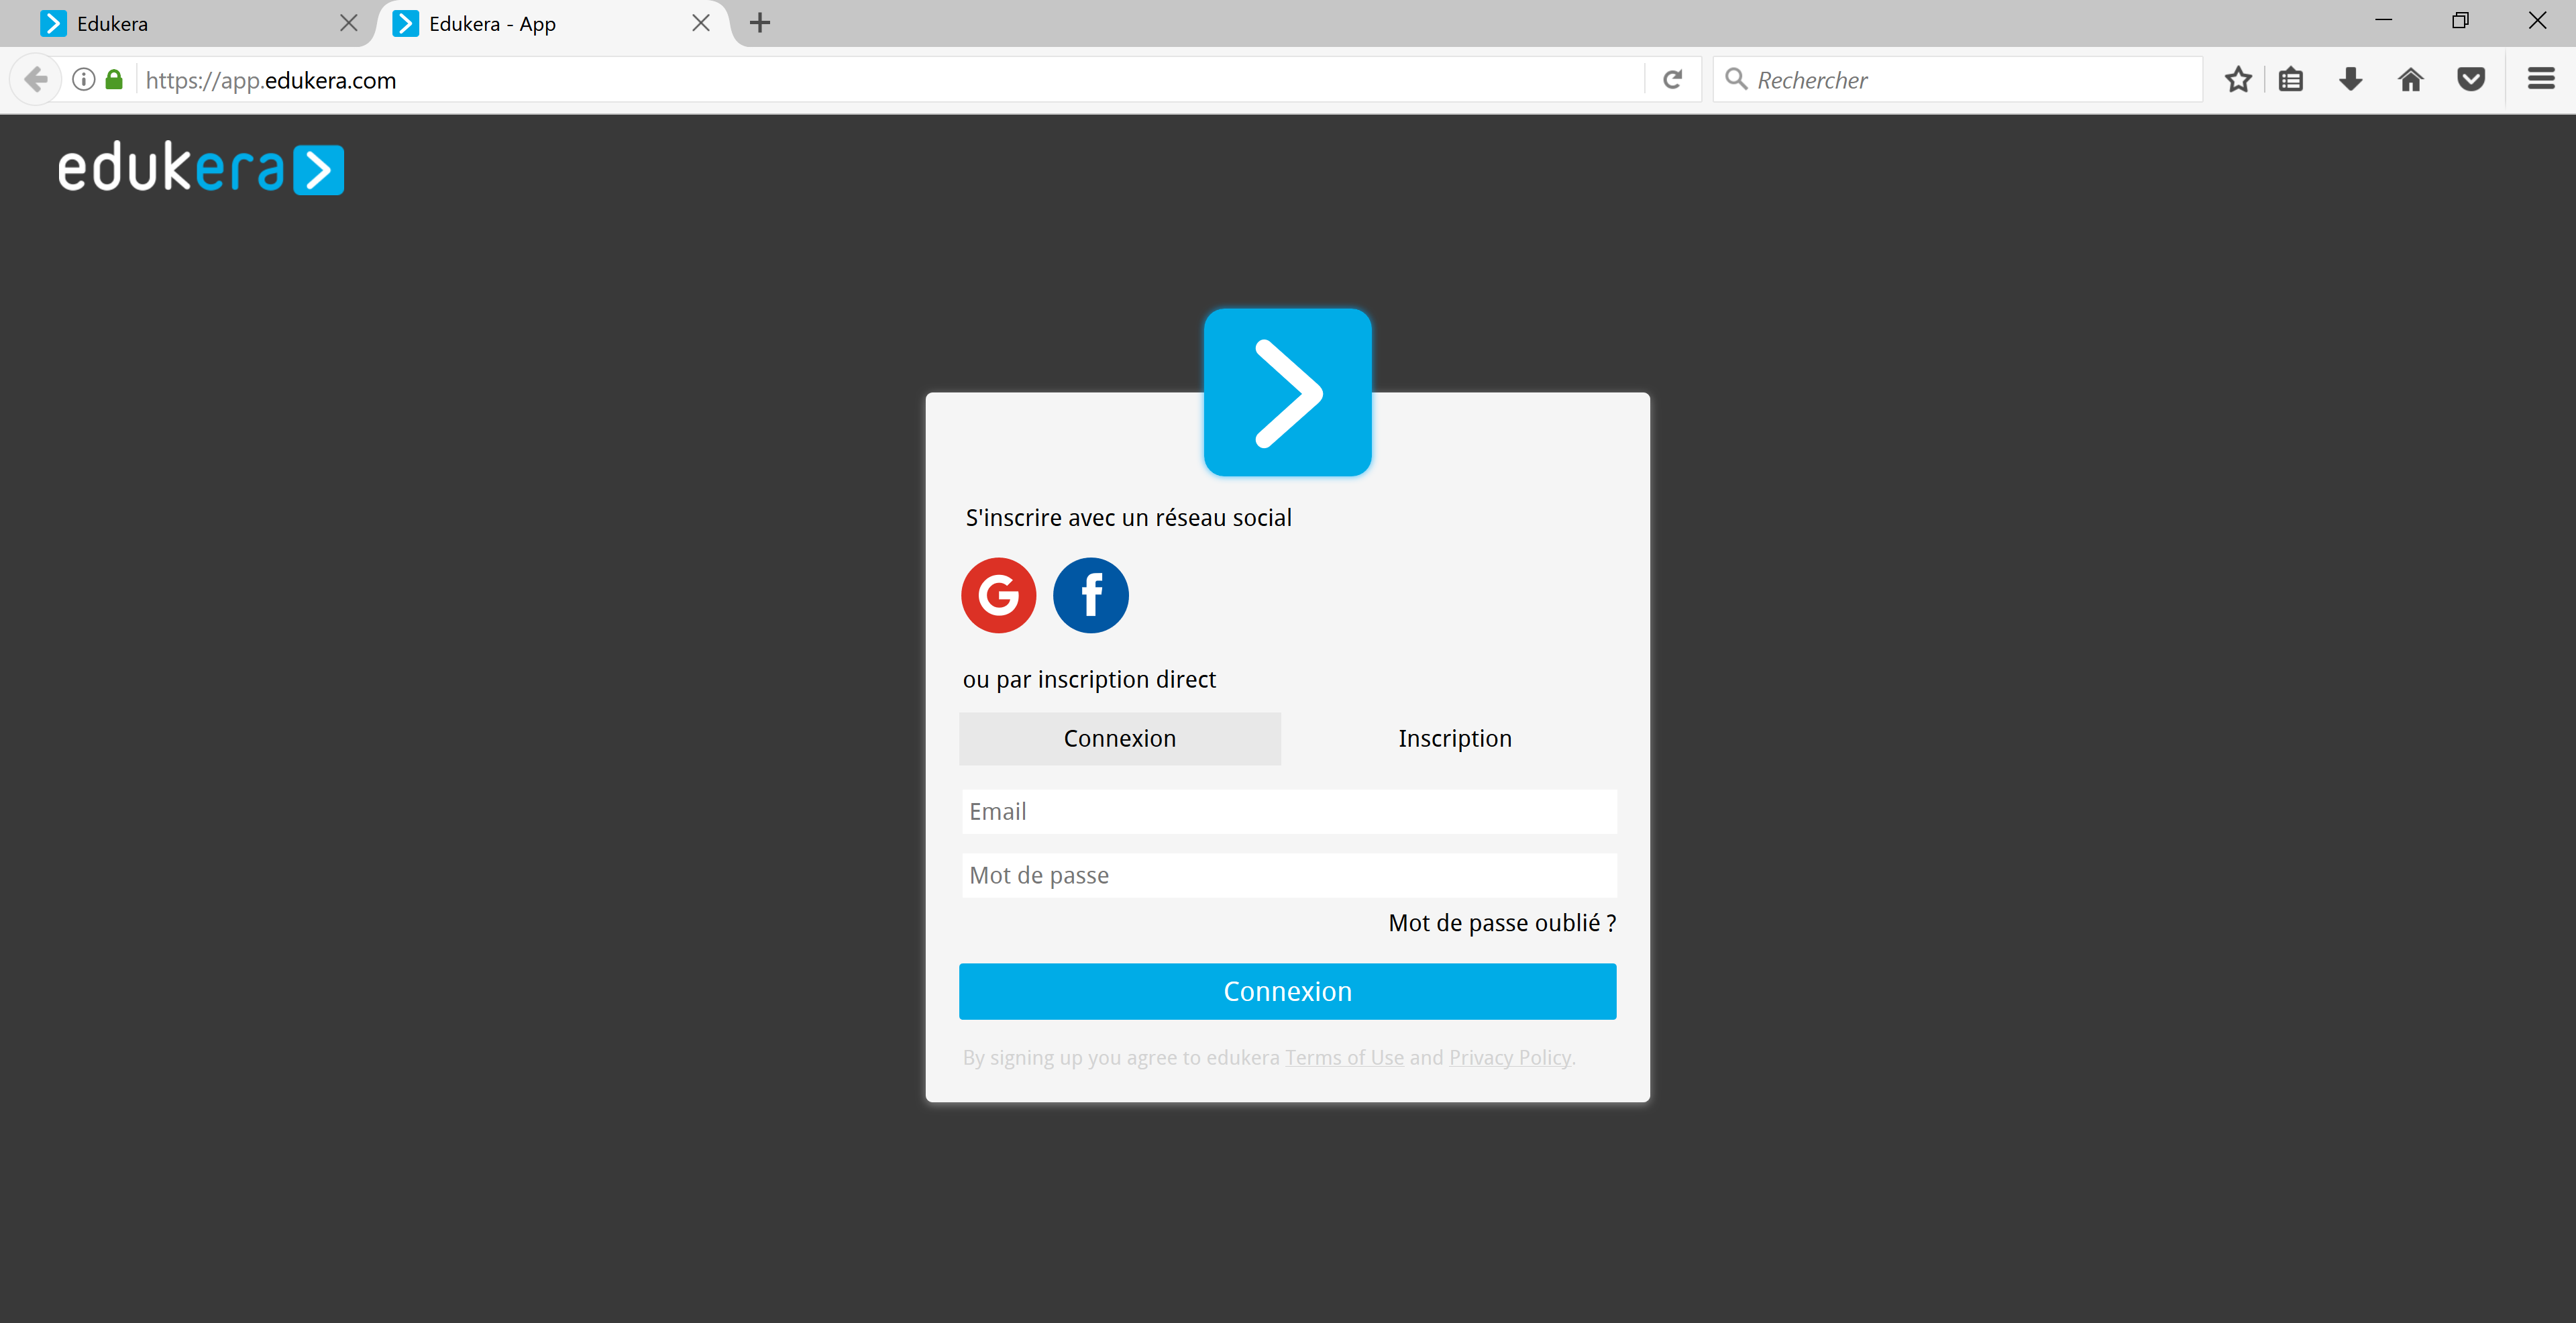
\includegraphics[scale=0.1]{img_site2.png}

Vous �tes maintenant pr�ts � faire votre premier exercice (enfin!).



\section{Faire son premier exercise}
\section{Devenir expert!}





\end{document}